\documentclass[dvipdfmx]{jarticle}
\usepackage{graphicx}
\usepackage[top=30truemm,bottom=30truemm,left=25truemm,right=25truemm]{geometry}
\usepackage{listings,jvlisting}
\usepackage{url}

\lstset{
  basicstyle={\ttfamily},
  identifierstyle={\small},
  commentstyle={\smallitshape},
  keywordstyle={\small\bfseries},
  ndkeywordstyle={\small},
  stringstyle={\small\ttfamily},
  frame={tb},
  breaklines=true,
  columns=[l]{fullflexible},
  numbers=left,
  xrightmargin=0zw,
  xleftmargin=3zw,
  numberstyle={\scriptsize},
  stepnumber=1,
  numbersep=1zw,
  lineskip=-0.5ex
}

\makeatletter
\newcommand{\subsubsubsection}{\@startsection{paragraph}{4}{\z@}%
  {1.0\Cvs \@plus.5\Cdp \@minus.2\Cdp}%
  {.1\Cvs \@plus.3\Cdp}%
  {\reset@font\sffamily\normalsize}
}
\makeatother
\setcounter{secnumdepth}{4}

\begin{document}
\begin{titlepage}
    \begin{center}
        {\huge 情報科学演習D 課題1レポ―ト}
        \vspace{180pt}\\
        \begin{tabular}{rl}
            氏名 & 山久保孝亮\\
            所属 & 大阪大学基礎工学部情報科学科ソフトウェア科学コース\\
            メールアドレス & u327468b@ecs.osaka-u.ac.jp\\
            学籍番号 & 09B22084\\
            提出日 & \today\\
            担当教員 & 桝井晃基 松本真佑
        \end{tabular}
    \end{center}
\end{titlepage}
\section{システムの仕様}
課題1で作成したプログラムの仕様は以下の通りである.
\begin{itemize}
    \item Pascal風言語で記述されたpasファイルを入力として,字句解析の結果であるtsファイルを出力する.また,開発対象のrunメソッドの第一引数はpasファイル,第二引数はtsファイルを指定する.
    \item  正常に処理が終了した場合は文字列"OK"を返し,入力ファイルが見つからない場合は文字列"file not found"を返す.
\end{itemize}
\section{課題達成の方針と設計}
課題1は字句解析と,解析したトークンをそれに対応する文字列とともにtsファイルに書き込む処理に分けられる.
\subsection{字句解析の処理}
字句解析の処理は以下のオートマトンに基づいて開発した.
\begin{figure}[h]
    \centering
    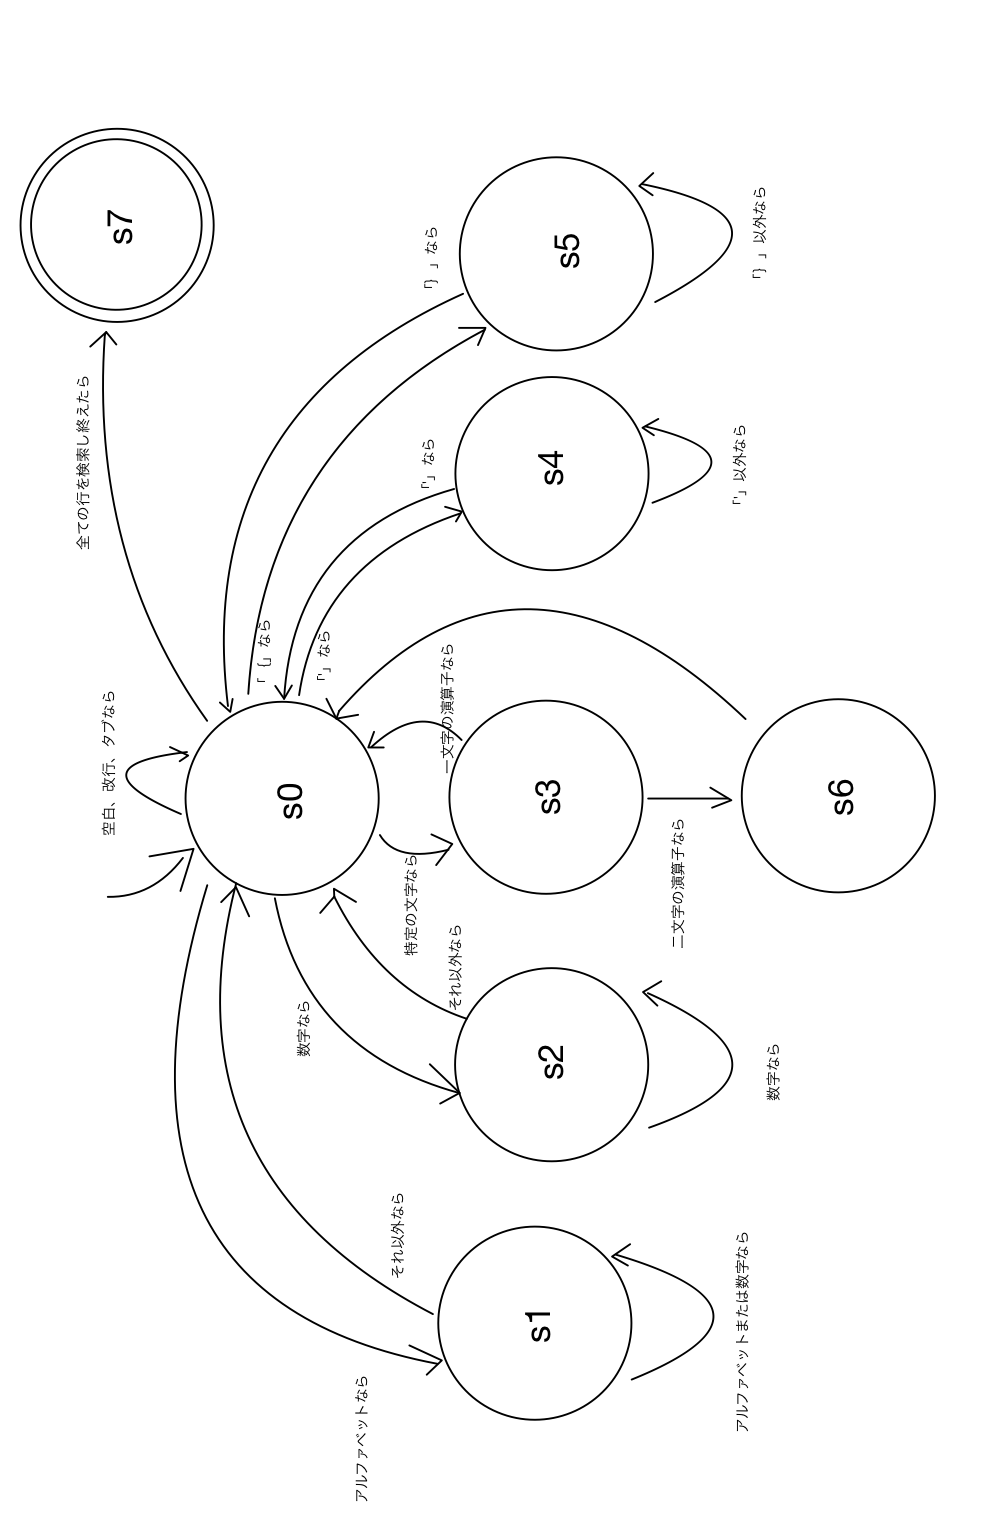
\includegraphics[width = 8cm, angle = -90]{automaton.png}
    \caption{字句解析部分のオートマトン}
\end{figure}
\\このオートマトンは合計8つの状態が存在し,初期状態はs0,受理状態はs7である.それぞれの有効辺の条件分岐は入力されたpasファイルの一文字について判定している.状態が変わるとその次の文字について調べ,pasファイルの最後の文字になると受理状態に遷移する.それぞれの状態においてs0に遷移する際にtsファイルに出力する処理を行う.
また,一字ずつ取り出す際にtoken\_loaded\_letterというリストを用いて,読み込み中のトークンの各文字を記憶しておく.そして,トークンの切れ目が確定してから各要素を合わせて文字列に変換する.その後token\_loaded\_letterは初期化する.
それぞれの状態の処理は3の実装プログラムで記述する.
\subsection{tsファイルに書き込む処理}
tsファイルに出力する処理を行うために,指導書に記載されている予約語とそのIDを格納するリストを事前に用意しておく.予約語が存在するソースコード中の字句をtoken,ソースコードに対応する予約語をtoken\_name,ソースコードに対応する予約語のIDをtoken\_idというリストにそれぞれ格納しておく.
そして,取り出したトークンがtokenの内いずれに当てはまるかについて判定しtoken\_nameとtoken\_idに格納されている対応する文字列を書き込む.
\section{実装プログラム}
2で記述した方針で作成するために,ここではpasファイルから文字を取り出す処理,字句解析のオートマトンのそれぞれの状態の処理,tsファイルへの書き込み処理の3つについて記述する.
\subsection{pasファイルから文字を取り出す方法}
pasファイルから各文字を一字ずつ評価するために,pasファイルから一行ずつ取り出し,各行から一字ずつ取り出す処理を行う.以下はその部分のプログラムを抜粋したものである.
\begin{lstlisting}
final List<String> buffer = Files.readAllLines(Paths.get(inputFileName));
while(i<buffer.size()) {
    String line = buffer.get(i) + "\n";
    while(j < line.length()) {
        char c = line.charAt(j);
        j++;
    }			
    i++;
 }
\end{lstlisting}
これによって,cにプログラムの各文字が格納されていくことになる.
\subsection{字句解析のオートマトンの処理}
まず図1のオートマトンの各状態に遷移するための条件分岐について記述する.3.1で取得したcについて評価してどの状態に対応するかを判定する.以下はその部分のプログラムを抜粋したものである.
\begin{lstlisting}
    //s0
    if(c == ' ' || c == '\t'|| c == '\n') {
    }else if(c == '{'){//s5
    }else if(c == '\'') {//s4
    }else if("/=<>+-*()[]:;.,".indexOf(c) !=-1){//s3
        if((c == '<'||c == '>'|| c == ':'|| c == '.')&&( j + 1 < line.length())) {//s6
        }else {//s3
        }
    }else if("0123456789".indexOf(c)!=-1){//s2
    }else {//s1
    }
\end{lstlisting}
この部分は3.1の二つのwhile文中に記述されているので,pasファイルの文字数分だけ実行される.また,"文字列".indexOf(c)は文字列中にcが含まれているかどうかを判定しており,
これで数字と特定の文字列が含まれているかを判定している.また,5行目のs3に遷移するかどうかを判定する際の文字列では,指導書の表6のトークン一覧に記載されていた記号を羅列したものでる.また,6行目のs6に遷移するかどうかを判定する際の文字列では,トークン一覧に記載されていた二文字の記号の内の一文字目を羅列したものである.
\subsubsection{状態1}
というリストを用いて,トークンを設定する.
\subsection{tsファイルに書き込む処理}
\section{考察や工夫点}
課題1において工夫した点は以下の二つである.
\begin{itemize}
    \item 一つ目はtoken,token\_name,token\_idの順番を対応させた点である.例えば,token,token\_name,token\_idの0番目にそれぞれand,SAND,0を格納したように,それぞれのリストのインデックスに対応する文字列を格納した.
    これにより,tsファイルに出力する際に取り出したトークンがtokenのどの要素に一致するかを調べるだけで,同じインデックスを使って字句解析機上でのトークン名とIDを取り出すことができた.また,divと\textbackslash はどちらも格納し,token\_nameでも同じトークン名で,token\_idでも同じIDで格納した.
    \item 二つ目はtsファイルに出力する処理をメソッドにしたことである.それぞれの状態からs0に遷移する際にトークンを主強くする必要があるので,メソッドにしないと同じ内容を繰り返し書くことになるので冗長になってしまう.これにより,プログラムの可読性を高めることができた.
\end{itemize}
\section{感想}
今回の課題を通して字句解析機の作成方法を学ぶことができた.符号なし整数と識別子の定義を間違えて認識していたので,デバッグの際に少し苦戦した.プログラムを記述する前にオートマトンの仕様を完全に決定できるとスムーズに開発が進むと感じた.
\section{謝辞}
今回の課題1にあたって質問対応してくださった教授,TAの方々,有難うございました.今後の課題もよろしくお願いします.
\begin{thebibliography}{1}
    \bibitem{1} 情報科学演習D指導書
\end{thebibliography}
\end{document}